% FIG-9.7: source-checked reconstruction V2, 2026-11-04.
\documentclass[border=5pt]{standalone}
\usepackage{fontspec}
\usepackage{unicode-math}
\setmainfont{Noto Sans}
\setsansfont{Noto Sans}
\newfontfamily\FigureItalic{Noto Serif}
\setmathfont{STIXTwoMath-Regular.otf}
\usepackage{tikz}
\usetikzlibrary{arrows.meta,calc,decorations.pathmorphing,decorations.markings,decorations.pathreplacing}
\definecolor{Ink}{HTML}{000000}
\definecolor{Curve}{HTML}{000000}
\definecolor{Muted}{HTML}{000000}
\tikzset{
 ax/.style={draw=Ink,line width=.72pt,-{Latex[length=2.3mm,width=1.45mm]}},
 lev/.style={draw=Ink,line width=1.50pt,line cap=butt},
 helper/.style={draw=Muted,line width=.65pt},
 bare/.style={draw=Muted,line width=.94pt,dash pattern=on 4pt off 2.5pt},
 curve/.style={draw=Curve,line width=1.85pt,line cap=round,line join=round},
 ray/.style={draw=Ink,line width=1.05pt,-{Latex[length=2.3mm,width=1.5mm]}},
 measure/.style={draw=Ink,line width=.85pt,{Latex[length=1.9mm,width=1.3mm]}-{Latex[length=1.9mm,width=1.3mm]}},
 flow/.style={draw=Ink,line width=1.05pt,postaction={decorate},decoration={markings,mark=at position .67 with {\arrow{Latex[length=2.3mm,width=1.5mm]}}}},
 link/.style={draw=Ink,line width=1.07pt},
 wave/.style={draw=Ink,line width=1.0pt,decorate,decoration={snake,amplitude=.34mm,segment length=2.7mm,pre length=1.0mm,post length=1.0mm}},
 lab/.style={text=Ink,font=\fontsize{14}{17}\selectfont,inner sep=2pt},
 small/.style={text=Ink,font=\fontsize{12.5}{15}\selectfont,inner sep=2pt},
 tag/.style={text=Ink,font=\fontsize{14}{17}\selectfont\FigureItalic\itshape,inner sep=2pt}}
\pagestyle{empty}
\begin{document}
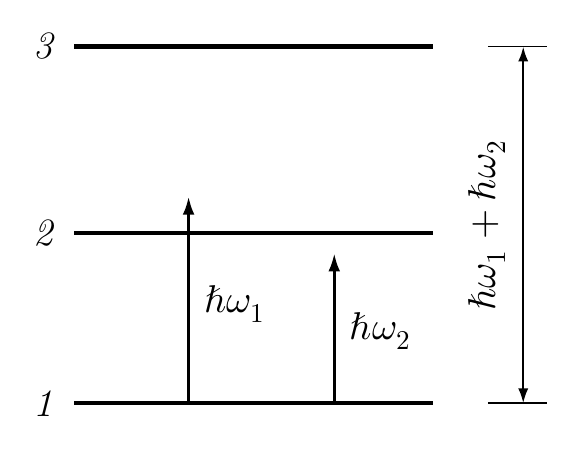
\begin{tikzpicture}[x=1cm,y=1cm]
% Figure 9.7, printed p.113. Illustrative energies; no measured scale.
% E3-E1 = hbar*w1+hbar*w2; virtual photon tips straddle real level 2.
\draw[lev] (1.250000,0.500000)--(5.800000,0.500000);
\node[tag,anchor=east] at (1.050000,0.500000) {1};
\draw[lev] (1.250000,2.663000)--(5.800000,2.663000);
\node[tag,anchor=east] at (1.050000,2.663000) {2};
\draw[lev] (1.250000,5.032000)--(5.800000,5.032000);
\node[tag,anchor=east] at (1.050000,5.032000) {3};
\draw[ray] (2.700000,0.500000)--(2.700000,3.126500);
\node[lab,anchor=west] at (2.820000,1.760720) {$\hbar\omega_1$};
\draw[ray] (4.550000,0.500000)--(4.550000,2.405500);
\node[lab,anchor=west] at (4.670000,1.414640) {$\hbar\omega_2$};
\draw[helper] (6.500000,0.500000)--(7.250000,0.500000);
\draw[helper] (6.500000,5.032000)--(7.250000,5.032000);
\draw[measure] (6.950000,0.500000)--(6.950000,5.032000);
\node[lab,rotate=90,anchor=south] at (6.800000,2.766000) {$\hbar\omega_1+\hbar\omega_2$};
\end{tikzpicture}

\end{document}
